\chapter{Potential Development and Pareto Optimality}
\label{ch:potential_development}

In the previous chapter, an overview of the different computational tools associated with atomistic simulation was presented to give some idea of the interconnectivity and breath of atomistic simulations.  In this chapter, we outline the Pareto approach to potential optimization within the context of more typical current appraoches to potential developmen so to understand the limitations of typical approaches.

Parameterization is often approached as the minimization of a scalar objective function consisting of the weighted sum of square differences with respect to the prediction of a set of material properties.  When the objective function is convex and continuously differentiable with respect to its parameters, scalar minimization approaches are relatively efficient, even in high dimensions.  For interatomic potentials, these conditions are most likely not guaranteed for even fairly simple formalisms.  When the scalar cost function is not convex, combining derivative-based local optimization procedures with global optimization techniques increases the complexity of parameterization and computational time even for a single selection of a weighting vector.

Moreover, gradient approaches to optimization are not amenable to parallelization.  Local optimization approaches are dependent upon an initial estimate of the optimal parameters and improve the estimate in an iterative manner.  As a result, the parallelization of the computational effort is limited by the dimensionality of the parameter space (length of the computation of the gradient) and limited to the number of simulations required to compute each material property.  This limits the processor utilization to $(M \times N_P)$, where $M$ is the number of simulations required to calculate the cost function, and $N_P$ is the dimension of parameter space.

A larger problem is that weighted least squares approach makes parameterization dependent upon the selection of weights and the choice of the initial condition, both of which heavily influence the final result and must be expressed \emph{a priori}. A potential developer is required to identifty weights before understanding what the trade-offs in performance are between alternatives.  Some methods have been developed to pre-determine weights, which incorporate the magnitude of acceptable errors of the target properties\cite{martinez2013_fitting}.  In practice, an initial choice of weights is made based on the experience of the potential developer, the weights are adjusted, and the optimization procedure repeated.  This process continues in an iterative fashion, until an acceptable parameterization is achieved.

To address the issues of this approach, a novel approach to parameter optimization is taken here which incorporates two pieces.  First, since gradient-based scalar optimization is problematic, we recast the problem as a multi-objective optimization problem (MOO), where each of the sub-objectives in the cost function is treated independently.  The concept of a single optimal parameterization is an inappropriate representation, since the improvement in the prediction in one material property generally causes a degradation in the prediction of another.  Each potential is optimal in its own way, a preference of one over an other is either subjective or dependent upon informatin not encoded into the problem, such as post-selection simulations to predict material properties that it was not optimized for.  Instead, the solution to a MOO is an ensemble of parameterizations; each optimal in its own way.  The performance of set of optimal potentials is defined as \emph{Pareto optimal surface} or \emph{Pareto surface}, and the set of parameterizations which produce these results are the \emph{Pareto optimal set}.  Second, while the Pareto set can be estimated by varying the weights in the cost function in a systematic way, such an approach is inefficient in the presence of local minima.  Instead, we propose that a weight-free, global-minimization approach based upon Monte Carlo sampling is a promising alternative to existing techniques.

This chapter consists of three sections.  In the first section, we introduce the idea of a potential energy surface and how interatomic potentials can be thought of as computationally inexpensive surrogate models; we also introduce the terminology of potential development as well as some broad concepts of potential optimization.

In the second section, we build up the notation and terminology of general optimization from a broad mathematical standpoint, first covering the more familiar single-objective optimization.  In particular, we discuss the current techniques which are applied to potential optimzation as well as some of the mathematical problems and issues of this approach.

In the third section, the problem of a parameterization is defined within the context of a MOO problem, with the solution of MOO being the sets of parameters, the Pareto set, which produce nondominated results in objective space, Pareto optimal surface.  When the Pareto surface is convex and continuously differentiable, gradient based approaches can estimate the Pareto surface.  When these conditions do not exist, gradient based approaches produces erroneous results.  As a preview to the evolutionary method presented in Chapter \ref{ch:methodology}, we demonstrate how a random sampling based approach to optimization is likely a better approach to estimating a Pareto optimal surface when the potential developer has a high degree of uncertainty to the selection of a region of potential parameterizations or weighting vectors.  This is demonstrated through some sample calculations the discontinuous, nonconvex MOO problem of Kurasawe\cite{kursawe1991_pareto}.

\section{Potential Energy Surfaces}

To study the evolution of a system, such as kinetic processes and chemical reactions, it is necessary to calculate the energy for every atomic arrangement of interest.  The potential energy surface (PES) is the energy of a collection of atoms as a function of the positions of its nuclei, $\{\bm{R}\}$.
A PES represents a mapping of the positions of the atoms of a material system to an energy, $V:\{\bm{R}\}\rightarrow E$, with $E\in\mathbb{R}$.
Given an atomic arrangement $\bm{R}$, the evaluated potential surface $V(\bm{R})$ gives the height of the energy landscape for any atomic configuration.
This creates an energy landscape which allows materials systems to be viewed from a topological perspective, that the PES can be used to describe the evolution of a system as it moves from one atomic configuration to another atomic configuration.

To describe empirical potentials, we provide with a a mathematical description of configuration space from a crystallographic perspective, and how this crystallgraphic perspective can be translated into other representations common with empirical potentials.

\section{Configuration Space}
\label{sec:configuration_space}
In solid materials, atoms are typically represented as infinite crystalline solids with atomic positions embedded within the representative unit volume.
This representative unit is referred to as a unit cell, which defines the periodic boundaries, the volume, and the lattice positions of each atom.

\begin{figure}[ht]
	\centering
  \includegraphics{chapter3/unit_cell}
  \caption{Depiction of the lattice vectors which bound the the unit cell depicted in blue.}
  \label{fig:unit_cell}
\end{figure}

The boundaries of the unit cell are defined by three lattice vectors, defined in three dimensional Euclidean space, $\mathbb{R}^3$.
The three lattice vectors, $\bm{a}_1$, $\bm{a}_2$, and $\bm{a}_3$, with $\bm{a_i}\in\mathbb{R}^3$, define a coordinate sytem in Euclidean space in which to describe a lattice.

To describe the atoms, each atom is identified by a chemical species, $s\in S$, and its atomic position, $\bm{r}$.
If the atomic positions are represented in the Cartesian unit vectors, $[\hat{\bm{\imath}},\hat{\bm{\jmath}},\hat{\bm{k}}]$, then the atomic positions are the ordered triplet, $(r_x,r_y,r_z)$.
More commonly, atomic positions, $(r_1,r_2,r_3)$, are represented in the coordinates system defined by the lattice vectors $[\bm{a}_1,\bm{a}_2,\bm{a}_3]$.  The transformation from the space described by the lattice space to Cartesian space, is described by equation.
\begin{equation}
	\label{eq:fractional_vs_cartesian_coordinates}
	r_x \hat{\bm{\imath}} + r_y \hat{\bm{\jmath}} + r_z \hat{\bm{k}}
	=
	r_1 \bm{a}_1 + r_2 \bm{a}_2 + r_3 \bm{a}_3
\end{equation}

The boundaries of the unit cell describes the periodic boundary conditions, since they also reflect that translational symmetry of the crystalline system.
Each lattice vector can be represented as a translational operator, $T_i$ for ${i\in\{1,2,3\}}$, such that, $T_i(\bm{r})=\bm{r} + n_i \bm{a}_i = \bm{r}$, and collectively,
\begin{equation}
    T(\bm{r}) = \bm{r}
		    + n_1 \bm{a}_1
		    + n_2 \bm{a}_2
		    + n_3 \bm{a}_3 = \bm{r}, \forall n_i \in \mathbb{Z}
\end{equation}

Thus, the geometry for a system with $N$ atoms can be described as
	$\bm{R} = \{\bm{a}_1,\bm{a}_2,\bm{a}_3,\bm{r}_1,...,\bm{r}_N\}$,
	where the $\bm{r}_i$ is defined in an coordinate system defined by the lattice vectors..

\subsection{Empirical Interatomic Potentials}

While the actual PES for any given material system is certainly not analytical, simulations based on solving the Kohn-Sham (KS) equations\cite{kohn1965_dft} of density functional theory (DFT)\cite{hohenberg1964_dft} can provide energy calculations of sufficient accuracy for many systems.  However, the computational bottleneck associated with solving for the charge density, energy levels, and wavefunctions of the KS equation limits its adoption as a viable energy calculator to systems consisting of no more than a few hundred atoms.

In contrast, the use of empirical interatomic potentials (EIP) in molecular dynamics simulations can routinely comprise of millions of timesteps on millions of atoms.  In \emph{ab initio} simulations, the solution to the electronic structure of the system is used to calculate the energies of atomic configurations and the forces on the atoms required to evolve the system. In contrast, EIPs have an analytical formalisms consisting of formulas which represent the relevant physics of the system.  This simplification in calculation allows energies and forces drastically improved computational efficiency at the expense of simulation fidelity.

The goal of developing an interatomic potential, $\hat{V}$, is to identify a computationally efficient surrogate model, which models the potential energy surface, $V$.  The use of a hat over a variable indicates that the quantity is an approximation of the actual value.
Since energy is a scalar value, both the PES ${V:\{\bm{R}\}\rightarrow \mathbb{R}}$ and and EIP ${\hat{V}:\{\bm{R}\} \rightarrow \mathbb{R}}$ are functions in the same space that assigns energies to atomic configuration.
The approximation relationship between the PES and the EIP is quantified the difference function $\epsilon$.
\begin{equation}
	\label{eq:pes_approximation}
    \hat{V}(\bm{R})
		=
		V(\bm{R}) + \epsilon(\bm{R}).
\end{equation}
In the above equation, $V(\bm{R})$ is the particular energy for a given atomic configuration $\bm{R}$, $\hat{V}(\bm{R})$ is the approximation of the interatomic potential for the same ${\bm{R}}$, and $\epsilon(\bm{R})$ is difference in energies between the two necessary to balance to the equation.

Interatomic potentials are often expressed as a series expansion of functional terms which explain the relevant physics of a system.  In these cases, the total energy of the system is sum of the individual contribution of each atom $i$.  For a system with $N$ atoms,
\begin{equation}
	\label{eq:potential_energy}
	\hat{V}(\bm{R})= \sum_{i=1}^{N} \hat{V}(\bm{r}_i)
\end{equation}
represents the potential energy of a system with $\hat{V}(\bm{r}_i)$ being the contribution of the $i$th atom of a system.
The total energy of a system with $N$ atoms interacting through the empirical potential, $\hat{V}$, can be expanded in a many body expansion as described in LeSar\cite{lesar2013_textbook}
\begin{align}
\label{eq:potential_expansion}
	\hat{V}(\bm{R}) &\equiv \hat{V}(\bm{r}_1,...,\bm{r}_N) \\
	          &= \sum_i V_{1,i} (\bm{r}_i)
	             + \sum_i \sum_{i<j} V_{2,(i,j)}(\bm{r}_i,\bm{r}_j)
		     + \sum_i \sum_{i<j} \sum_{j<k} V_{3,(i,j,k)}(\bm{r}_i,\bm{r}_j,\bm{r}_k)
		     + ...
\end{align}
Based upon this expansion, we can classify certain potentials into three classes: pair-potentials, three-body potentials, and many-body potentials.

The first term $V_1$ is the one body term, due to an external field or boundary conditions, which is typically not needed in classical potentials.  The second term $V_2$ is the pair potential; the interactions of this term is dependent the upon the distance between two atoms $\bm{r}_i$ and $\bm{r}_j$, and it is common to represent the distance between the two atoms as $r_{ij}=\lVert \bm{r}_i - \bm{r}_j \rVert^2$.  The three-body term potential $V_3$ arises when the interaction interaction of a pair of atoms is modified by the presence of a third.  In these cases, the pair-potential is typically augmented with three-body terms to express angular dependence, with $\theta_{ijk}$ typically represnting the angle formed by atoms $j$ and $k$ around the central atom $i$\cite{stillinger1985_sw}.  Few potentials employ four-body terms due to the dramatic expansion in terms required to describe the interaction.  Instead, a many-body interations is used to reflect the local environment around the atom $i$.

Not all potentials have the decomposition described in Equation \ref{eq:potential_expansion}.  For example, the embedded atom method (EAM)\cite{daw1984_eam} is a popular approach for modeling metals in molecular dynamics simulations.  In metallic systems, an atom is embedded in a sea of delocalized electrons contributed by its neighbors.  To capture this physics, Daw and Baskes postulated a potential which consisted of the pair-wise interactions of the nuclei and an embedding energy term as a function of the host electron density created by all the other atoms in the system.  The EAM model clearly can notbe written in the expansion implied by Equation \ref{eq:potential_expansion} without including very high-order terms, but can be compactly represented by a pair-function and an embedding energy functional dependent upon the pair-wise density contributions defined by density function.

\begin{figure}[h]
  \centering
    \includegraphics[width=5in]{chapter3/lj}
    \caption[The Lennard Jones Potential]{The Lennard Jones potential with $\sigma=1.0$ and $\epsilon=1$, which correspond to the location and depth of the energy well respectively.}
		\label{fig:lj_potential}
\end{figure}

A set of equations, collectively referred to as a formalism, compromises an analytical potential, which decomposes the energy of an atomic configuration into the individual contributions of the terms.
One analytical formalism can be used to describe different chemical compositions with similar underlying physics.  A process of parameterization specializes these functional forms to the specific composition of chemical species, through a process known as parameterization.
If $\hat{V}(\bm{R}:\bm{\theta})$ represents an empirical interatomic potential and is parameterized by a vector of parameters, $\bm{\theta}=(\theta_1,...,\theta_n)$, then $\hat{V}(\bm{R}:\bm{\theta})$ approximates $V(\bm{R})$.

The selection of parameters for the Lennard-Jones (LJ)\cite{lennardjones1924_lj_pot} potential demonstrates a simple process for the selection of parameters. The LJ potential approximates the interaction between a pair of neutral atoms, such as a noble gas.  The LJ potential is
\begin{equation}
	V_{\text{LJ}}(r_{ij}) = 4 \epsilon
    \left[
	\left(\frac{\sigma}{r_{ij}}\right)^{12}
	- \left(\frac{\sigma}{r_{ij}}\right)^{6}
    \right].
\end{equation}
The $r^{-12}$ term is repulsive due to the Pauli exclusion principle, which describes overlapping electron orbitals.  The $r^{-6}$ is the attractive long range term, describing the attraction at longer ranges from van der Waals forces.  This equation has two parameters, $\sigma$ and $\epsilon$, which can used to reproduce experimental experimental data or \emph{ab initio} calculations.  As depicted in Figure \ref{fig:lj_potential}, $\sigma$ controls the location of potential well, which is correlated to latttice parameter predictions while $\epsilon$ controls the magnitude of the interatomic interactions, controlling properties like cohesive energy.


\section{Traditional Approaches to Potential Deveopment}

In the typical use of a potential, the parameters are considered to be fixed, $\hat{V}(\bm{R}|\bm{\theta})$, and the function is considered to vary only with respect to the configuration of atoms, $\bm{R}$.  In determing the potential parameterization, the empirical potential is treated as varying with respect to the parameterization, $\bm{\theta}$, while keeping the set of atomic configurations fixed $\bm{R}$.

The process of determining the optimal parameterization, $\bm{\theta}^*$, for $\hat{V}(\bm{R}|\bm{\theta})$ is a process called fitting, which is a process of constructing a curve that has the best fit to a series of data points.  Given an EIP functional form,  the ordinary least squares approach is to minimize the square differences between $\hat{V}(\bm{R}|\bm{\theta})$ and $V(\bm{R}_i)$ over configurational space,
\begin{equation}
\label{eq:energy_matching}
	\bm{\theta}^*
		= \argmin_{\bm{\theta}\in\bm{\Theta}}
					\sum_i \left(\hat{V}(\bm{R}_i|\bm{\theta}) - V(\bm{R})\right)^2
\end{equation}
where $\bm{\Theta}$ being the set of all possible parameterizations and over each atomic configurations $i$.  Since the set of possible atomic configuration $\{\bm{R}_i\}$ is countably infinite, the interatomic potential has to be developed from a finite set of reference configurations, $\{\bm{R}_i:i<N_{C,F}\}$, which known as the fitting set.  To ensure that $\bm{\theta}^*$ is transferrable to configurations not part of the fitting set, an additional set of configurations $\{\bm{R}_i:i<N_{C,T}\}$ are necessary to  to test $\bm{\theta}^*$ against. For notational convenience, $N_C$ will refer to the number of structures in the fitting set.

\section{Force Matching Method}
Using \emph{ab initio} simulations as the representation of the PES ($V(\bm{R})=\hat{V}_{\text{DFT}}(\bm{R})$), a sequence of atomic configurations can be generated.  Typically, a DFT code is used to calculate energies for the atomic configuration and the interatomic forces for each atom in that atomic configuration. Since both energy and forces data are generated in these simulations, the energy matching method described by Equation \ref{eq:energy_matching} can be augmented with a force matching method of Ercolessi and Adams\cite{ercolessi1994_fitting_forcematching}, where they define the objective function,
\begin{equation}
\label{eq:force_matching}
	C_{F}(\bm{\theta}) = \left(3\sum_{k=1}^{N_C} N_k \right)^{-1}
		\sum_{k=1}^{N_C}\sum_{i=1}^{N_k}
			\Vert \hat{\bm{F}}_{ki}(\bm{\theta}) - \bm{F}_{ki}\Vert^2.
\end{equation}
where $N_k$ is the number of atoms in configuration $k$, $\hat{\bm{F}}_{ki}(\bm{\theta})$ is the force on the $i$th atom in set $k$ obtained from the parameterization $\bm{\theta}$, and $\bm{F}_{ki}$ is the reference force from the first principles calculation.

In this approach, the fitted potential becomes a surrogate for the potential energy surface estimated by the \emph{ab initio} approach, biasing the parameterization to replicate any errors that may manifest itself due to the first principles method, such as the choice of the exchange correlation functional.  For example, it is well-known that local density approximation (LDA)\cite{kohn1965_dft} calculations tend to result in overbinding causing an underestimate of the lattice constants and an overestimate in the cohesive energies, phonon frequencies and elastic moduli\cite{vandewalle1999_lda_overbinding}.  The generalized gradient approximations (GGA) corrects this error.  The most ubiquitous GGA functional, by Perdew-Burke-Ernzerhof (PBE)\cite{perdew1996_gga_pbe} is known to overcorrect, as analyzed by Wu and Cohen\cite{wu2006_gga_underbinding}.  Moreover, there is not yet a reliable way to estimate their errors beyond the empirical observation that LDA and GGA results generally span experimental values for many structural and mechanical properties.

The force matching and energy matching approach is popular for the development of modern machine learning potentials which have no functional form, but a complicated mathematical formalism with hundreds of parameters\cite{behler2016_ml_pot} which requires a large number of datapoints to prevent overfitting\cite{wood2018_snap}.

\subsection{Fitting Database}

For analytical potential development, particularly with less complicated functional forms, the computational investment required to acquire such large \emph{ab initio} datasets is unncessary.  Instead, the typical approach to potential development is to match the prediction of materials properties to reference values.  In this approach,  potential development comes from optimizing a potential based upon the performance to a fixed set of material properties, known as the fitting database.

In this approach, materials properties are directly related to quantities of interests (QOIs) chosen by the potential developer.  The term QOI comes from the field of verification, validation, and uncertainty quantification (VVUQ), where the parametric uncertainty of a model propagates to create uncertainty in the predictions of the QOIs.  Contrariwise, if the uncertainty with respect to a QOI could also be used to determine the parametric uncertainty of a model due to uncertainty in the fitting data.   Adopting this notation, material properties are denoted  $\bm{q} = ( q_{1},...,q_{N_Q} )$, for $N_Q$ quantities of interest (QOIs); the values predicted by a potential are denoted, $\hat{\bm{q}}= (\hat{q}_{1},...,\hat{q}_{N_Q})$.

A fitting database is a collection of structure-property functions $q_i$ associated with specific atomic configurations.	The calculation of the $i$th QOI from atomistic simulation tools can be decomposed as a function of energy evaluation of the PES over the $N_{C,i}$ atomic configurations required to do the calculation,
	\begin{equation}
		q_i = q_i(\bm{R}_1,...,\bm{R}_{N_{C,i}}).
	\end{equation}
Likewise, the prediction of the QOI from a formalism, can likewise be denoted as
	\begin{equation}
		\hat{q}_i(\bm{\theta})
		=
		\hat{q}_i(\bm{\theta}|\bm{R}_1,...,\bm{R}_{N_{C,i}}).
	\end{equation}
The choice of the more compact notation indicates that once the fitting database is fixed, $q_i$ becomes a static value and $\hat{q_i}(\bm{\theta})$ becomes a function only dependent upon the vector of parameters.

Unlike force matching techniques which require a consistent set of electronic structure data to prevent numerically inconsistent data\cite{behler2016_ml_pot}, a reference value $\hat{\bm{q}}$ can be taken from experiment, calculated from \emph{ab initio} techniques, or integrated from calculations at different levels of theory.  In early efforts of potential development, potentials were developed by fitting to a few experimental numbers.	Due to the increased confidence in DFT calculations, the current trend is to include a significant amount of \emph{ab initio} data.

Since DFT determines the ground state electronic structure, incorporation of these reference values into the fitting database allows fitting to structural properties which are experimentally difficult to access, such as information from kinetically unstable structures.  The incorporation of first-principles data in the fitting database significantly improves the reliability of EIPs by sampling a larger area of configuration space; this is discussed in detail in the review article by Payne \emph{et al}.\cite{payne1996_dft_database}

From a computational standpoint, at $0 \,\mathrm{K}$  the calculation of material properties become precise because atomic motion stops, and only a single evaluation of a parameterization needs to be evaluated against the reference value.  When the $T>0 \,\mathrm{K}$, time integration through molecular dynamics is necessary to calculate these QOIs.  Shorter trajectories yield incomplete information and confound comparison of parameters with experimental values.  When many $\hat{\bm{q}}(\bm{\theta})$ have to be evaluated many times, fitting to structure property relationships which are dependent upon themodynamic ensembles quickly becomes computational infeasible.

The goal of a fitting database is to find a representative set of structures in which to calculate the structure property relationships $q_i$.  Since $q$ is ultimately detemined from simulations on a series of atomic configurations, we can represent the energy difference between the predicted QOI and the target QOI,
\begin{equation}
	\epsilon(\bm{\theta})=\hat{q}(\bm{\theta})-q
\end{equation}
By choosing a set of QOIs, the number of structures in the fitting database is effectively fixed.  In turn, the the computational investment required to creating the the fitting dataset is reduced, when QOIs are determined by DFT.  In addition, the time required to evaluate a parameter set is likewise reduced, an important consideration when $\hat{\bm{q}}(\bm{\theta})$ is evaluated tens of thousands of times against different parameters $\bm{\theta}$.  The collection of structure-property relationships is denoted $\bm{q}=(q_1,q_2,...,q_{N_Q})$ for $N_Q$ structure-property relationships.

The determination of the optimal fitting database is a current area of interest\cite{zhang2015_bayes_fitttingdb}.  When the fitting database is defined, potential development then proceeds by the determination of the optimal parameterization $\bm{\theta}^*$.  With the description of the fitting database achieved, our discussion turns on how this potential database can be used to obtain $\bm{\theta}^*$.

\subsection{Cost Function}
\label{subsec:cost_function}

Typically, the squared difference between the predicted material property values and reference values, $\epsilon_i^2=(\hat{q}_i(\bm{\theta})-q_i)^2$, is used to measure the error since these quantities are analogous to the statistical measure of variance around a mean. The goal of fitting can be described as the selection of a parameter set which minimizes all error terms,
\begin{equation}
\label{eq:moo_LS}
	\min_{\theta\in\Theta}
		  \quad  (\hat{q}_i(\bm{\theta})-q_i)^2,
						\quad i = 1,...,N_Q
\end{equation}

Since analytical formalisms preserve only the salient physics of a particular system, it is inevitable that the potentials will have limitations in their predictive performance caused by the inadequacies of $\hat{V}$ to faithfully replicate $V$.  It is not usually possible to minimize all error terms simultaneously as there are almost inevitably tradeoffs in which reducing the error for one QOI increases the error in another QOI.  This problem is a classic problem in multiple criteria decision-making where more than one objective function needs to be optimized simultaneously\cite{miettinen1998_mcdm}.  In fitting interatomic potentials, optimal decisions need to be taken in the presence of trade-offs between conflicting objectives.

One approach to solving this problem is the use of a response data transformation to recast a multi-objective problem as a single-objective problem.  The typical approach is to couple these objective functions with a weighted sum of squares known as the cost function. Thus, instead of multiple objective functions we have a single objective function to minimize
\begin{equation}
	\label{eq:cost_function_LS}
	C(\bm{\theta})
	=\sum_{i=1}^{N_Q}
	      w_i(\hat{q}_i(\bm{\theta})-q_i)^2
	=\sum_{i_1}^{N_Q}
	      w_i \epsilon_i^2(\bm{\theta})
\end{equation}
In this equation, the weights, $w_i$, represent the preferences of the potential designer and effectively serve as the “knobs” which allow control of the parameterization. For example, for the proposed applications of the potential, obtaining precise agreement with the elastic properties may be more important than optimizing the point defect energetics or, of course, vice versa. Although the values of $w_i$ are not explicitly defined in the interatomic potential, $\hat{V}(\bm{R}|\bm{\theta})$, they clearly play a strong role in determining the optimized parameter set.  Since the values of $w_i$ are determined by the potential designer, they are in a sense arbitrary as they reflect subjective preferences upon which the model prioritizes fidelity of one material property at the expense of another.

When $\bm{w}$ is static, UQ techniques were pioneered by Frederiksen \emph{et al.}\cite{frederiksen2004_md_bayes}, where uncertainty in the parameters were estimated from $T > 0K$ simulations using \emph{ab initio} molecular dynamics as reference target values contained aleatory certainty.  However, as $T \rightarrow 0 $ K, uncertainty of the parameters decreases and vanishes to the model fit to the $0$ K reference values.  This should not be surprising as UQ techniques require expressing the uncertainty associated with each $q_i$ with a probability distribution function.  For $0$ K reference values, the aleatory uncertainty disappears and what is typically left is the epistemic uncertainty associated with \emph{ab initio} reference calculations, which cannot be meaningly quantified into a probability distribution, since the reference values in the fitting database are point estimates.

Given a potential formalism, potential developers produce different parameterizations based upon fitting databases which are more similar than they are different.  The real uncertainty in potential development is driven by the choice of $\bm{w}$.  The choice of $\bm{w}$ is nontrivial, considering that this decision must be made \emph{a priori} and the potential developer may not know the implications of adverse changes in prioritizing performance of a potential for a particular material property.

Martinez \emph{et al.}\cite{martinez2013_fitting,martinez2016_posmat} describe an approximation procedure which normalizes the $w_i$ by $q_i$ and multiplies by magnitude of the acceptable fractional error.  Starting with an initial estimate of the optimal parameterization $\bm{\theta}_0$ and an initial weighting vector $\bm{w}_0$, an initial parameterization is achieved through a combination of gradient descent and global optimization techniques, resulting on an "optimal" paramaterization, depending on the choice of initial conditions, weight preferences, and choice of minimization methods.  Often this result is not acceptable, so an \emph{ad hoc} adjustment is applied to the weights, and the process continues iteratively until an acceptable potential is acquired.  Typically, these details are not provided in literature, hindering reproducibility of the potential development process.

When the weighting scheme is used as an \emph{a priori} method, the potential developer is expected to represent his/her preferences in the form of weights.  Roy and Mousseau\cite{roy1996_moo_weights} suggests that the role of weights in expressing preferences may be misleading.  Although the relative importance of weights shows the relative importance of the objective functions, it is not clear what underlies this notion.  The relative importance of an objective function is usually understood globally, for the entire decision problem, while many practical applications show that the importance typically varies for different objective function values; that is, the concept is only meaningful locally\cite{podinovski2002_moo_weights}.

Additionally, the minimization of the cost function is no guarantee of transferability.  A potential which is transferable can describe material properties and structures which are different from those it was fitted to.  In some general sense, the issue of transferability deals with the problem of overfitting as well as capturing the relevant physics with the correct functional form.  To assess transferability, a potential needs to adequately describe atomic configurations which are substantially different from those contained in the training set as well as material properties not in the training set.  Moreover, the parameterization of an empirical potential should be relatively insensitive to small changes in weights in the cost function\cite{martinez2013_fitting}.

\section{Optimization and Pareto Efficiency}

With the context provided by the typical approach to potential development described above, the attention of the rest of this chapter now turns to the development of a more general framework for describing the problem, and the representation of the solution of the problem as Pareto set.  In Section \ref{subsec:cost_function}, multi-objective optimization was introduced by coupling the many objective functions in Equation \ref{eq:moo_LS} into a single cost function in \ref{eq:cost_function_LS}.  Adapting the notation of Marley and Arora\cite{marler2004_moo_survey}, the general statement of for the potential parameterization is
\begin{subequations}
	\label{eq:moo}
\begin{align}
  	&\min_{\bm{\theta}}
	    & & \bm{L}(\bm{\epsilon}(\bm{\theta})) \\
    &\text{subject to}
	    & & g_{\Theta,j}(\bm{\theta}) \leq 0,
			    \; j=1,2,...,N_g \\
	  & & & h_{\Theta,k}(\bm{\theta}) = 0,
		      \; k=1,2,...,N_h \\
	  & & & g_{Q,m}(\hat{\bm{q}}(\bm{\theta})) \leq 0,
		      \; m=1,2,...,N_m
\end{align}
\end{subequations}
where
$N_g$ is the number of $g_\Theta$ inequality constraints on the parameters,
$N_h$ is the number of $h_\Theta$ equality constraints on the parameters,
and $_m$ is the number of $g_Q$ inequality constraints on the QOIs.
Here,
$
\bm{L}(\bm{\epsilon}(\bm{\theta}))
=
[
  L_1(\epsilon_1(\bm{\theta})),
	...,
	L_{N_Q}(\epsilon_{N_Q}(\bm{\theta}))
]
$ are the loss functions, which are a measure of the information loss of a potential.  This concept is discussed in more detail in Section \ref{sec:loss_functions}.  For now, let us assume that $L$ is a monotonically increasing function with respect to $|\epsilon_i|$ for $|\epsilon_i| \geq 0$ with $L(\epsilon_i)=0$ when $\epsilon_i=0$.

In MOO literature, the vector $\bm{\theta} \in \bm{\Theta} \subseteq \mathbb{R}^{N_P}$ is a vector of the design variables $\bm{\theta}_i$, for $i=1,...,N_P$, and $\bm{\Theta}$ is feasible design space.  $\bm{L}(\bm{\theta}) \in \mathbb{R}^{N_Q}$ are called objectives, cost functions, or criteria.

The best parameterization $\bm{\theta}^* \in \bm{\Theta}$ minimizes a set of objective functions, which we take here to be a set of loss functions, $\bm{L}=\{L_1,...L_{N_Q}\}$.  When $N_Q=1$ the problem is a single objective optimization problem and the goal is to find the optimal potential $\bm{\theta}^*$ that minimizes a single loss function $L$, i.e.,
\begin{equation}
	\bm{\theta}^* = \argmin_{\bm{\theta}\in\bm{\Theta}} L(\bm{\theta}).
\end{equation}
When $N_Q>1$, the problem becomes a multiple-objective optimization problem(MOO).

In multiobjective optimization problems, it is characteristic that no unique solution exists, but a set of mathematically equally good solutions can be identified.   Such a set of solutions are really trade-offs or good compromise solutions among the objectives.  In other words, a solution to a MOO problem is Pareto optimal if there exists no other feasible solution which would decrease the error in some criterion without causing a simultaneous increase in the error of at least one other criterion. The use of this concept almost always gives not a single solution $\bm{\theta}^*$ but a set of them $\{\bm{\theta}^*\in \bm{\Theta}^* \subseteq \bm{\Theta}\}$.  These solutions are known as nondominated, efficient, noninferior or Pareto optimal solutions.  In MOO literature, these terms are synomous.  A more complete discussion of Pareto optimality is in Section \ref{sec:pareto_efficiency}.

\subsection{Loss Functions}
\label{sec:loss_functions}
The loss function
$L_i(|\epsilon_i(\bm{\theta})|)$ describes the information loss for the $i$th QOI is a function of the absolute difference between predicted and target values.  In machine learning strategies, literature will often refer to its negative, the fitness function, which indicates the system of equations is to maximized rather than minimized.  Throughout this work, the objective functions will be expressed as minimization functions.

The absolute difference function,
\begin{equation}
	\label{eq:L1_loss_function}
	L_1(\bm{\theta})
	= |\epsilon_i(\bm{\theta})|
	= |\hat{q}_i(\bm{\theta})-q_i|
\end{equation}
has the benefit in that it is in same units as $q_i$.  However, when using gradient techniques, $L_1$ is not continuously differentiable at the area of interest (i.e. where $\epsilon_i =0$), which likely will create numerical instability problems.

The cost function of Equation \ref{eq:cost_function_LS} uses the quadratic loss function
\begin{equation}
	\label{eq:L2_loss_function}
  L_2
	=\epsilon(\bm{\theta})^2
	=(\hat{q}_i(\bm{\theta})-q)^2.
\end{equation}
$L_2$ has the benefit of being a continuously differentiable concave function with respect to $\hat{q}(\bm{\theta})$, which is desirable property in optimization algorithms dependent upon numerical derivatives.  However, the continuity and convexity $L^2$ with respect to $\bm{\theta}$ is not guaranteed, and is dependent upon to the continuity and convexity of $\hat{q}(\bm{\theta})$ with respect to $\theta$.

Depending upon optimization routine, different loss functions may give different results given the same weighting scheme.  For example, optimization of the cost function using $L_1$ will give different results than an optimization based upon $L_2$, because $L_2$ increases quadratically with respect to $|\epsilon_i(\bm{\theta})|$.  In the algorithm presented Chapter \ref{ch:methodology}, the results do not change because $L_1$ and $L_2$ produce the same ordinality of information loss.

The choice of a loss function is not arbitrary.  Typically, the choice of the loss function is based on convenient mathematical properties such as symmetry and continuous differentiability to make the loss function compatible with the optimization algorithm.  For example, a potential developer might want to choose an asymetrical loss function to penalize parameters where $\epsilon_i(\bm{\theta}) > 0$ different than $\epsilon_i(\bm{\theta}) < 0$ if there is a clear preference for upside vs. downside errors.

For the purposes of this work, an acceptable cost function $L$ must be postive and $L$ must preserve the order with respect to $L_1$.   $\bm{\theta}_i$ and $\bm{\theta}_j$, if $|\epsilon(\bm{\theta}_i)| < |\epsilon(\bm{\theta}_j)|$, then $L(\bm{\theta}_i) < L(\bm{\theta}_j)$.

\subsection{Parameter Constraints}

Since analytic formalas respect the relevant physics of a system, the parameters of the formulas may have physical meaning.  An optimal parameter should represent realistic physics, such as the coefficients of attractive and repulsive terms having the correct sign.  These can be encoded as inequality constraints to enforce $\bm{\theta} \in \bm{\Theta}$.

Moreover, it may also be desirable to impose equality constraints on certain parameters.  In charged systems, it is desireable to preserve charge balance.  For magnesium oxide (MgO), it is necessary to balance the charges between magnesium and oxygen ions.  This equality constraint can be expressed as $Z_{\text{Mg}} = -Z_{\text{O}}$.

Finally, we want to impose constraints upon QOIs.  For example, the formation energy for the ground state atomic configration (in eV/atom) should be the minimum on the convex hull for competing phases.  Otherwise it would decompose into other compounds with lower energies.  For nickel, the face-cented cubic (FCC) structure is the expected ground state.  In addition to fitting the phase energy difference between FCC and the competing phase, it is also desireable to impose the restriction that the phase energy difference is positive between FCC and other structures such as BCC, HCP and diamond cubic.

\subsection{Pareto Efficiency}
\label{sec:pareto_efficiency}

To address the problem of weights, a further discussion of Pareto efficiency is necessary. This concept was first introduced by Vilfredo Pareto to model the allocation of resources in an economy\cite{pareto1897_pareto}.  Pareto was the first to realize that cardinal utility could be dispensed with and be replaced with ordinal utility\cite{aspers2001_pareto}.  Cardinal utility corresponds to scalar optimization.  Ordinal utility ranks options in terms of preference; order is imposed.  For any two points, $A$ and $B$, exactly one of the following is true: $A$ is preferred to $B$ (i.e. $A$ dominated $B$), $B$ is preferred to $A$ (i.e. $B$ dominates $A$), or one is indifferent between the two points(e.g. both points are mutually non-dominated).

As a result, the notion of total aggregate utility to represent the greatest good for the greatest number of people is replaced in modern economic with the notion of Pareto optimality, the idea that a system is maximized when no one can be made better off without making someone else worse off\cite{mathur1991_pareto}.

Likewise, in the field of potential development, the use of a cost function unnecessarily constrains potential development, encoding a subjective performance preferences by assigning a vector of weights to correspond with the vector of sum squared errors.  This is ultimately a subjective determination by the potential developer, who is ultimately unable to express these preferences \emph{a priori} because knowledge in the relative tradeoffs is necessary to make an informed decision.  Instead of determining $\bm{\theta}^*$ with a cardinality loss function, which aggregates the subobjective functions, one can calculate the Pareto surface to determine $\bm{\Theta}^*$.  Since these potentials are Pareto efficient, the decision then becomes choosing $\bm{\theta}^* \in \bm{\Theta}^*$.

A system with $N_Q$ QOIs has a equal number of objective functions.  Since all objective functions are to be minimized, a feasible parameterization $\bm{\theta}_1$ is said to dominate another feasible parameterization $\bm{\theta}_2$, if and only if $L_i(\bm{\theta}_1) \leq L_i(\bm{\theta}_2)$ for $i = 1,...,N_Q$ and $L_j(\bm{\theta}_1) < L_j(\bm{\theta}_2$) for at least one objective function $j$.  A solution is said to be Pareto optimal if it is not dominated by any other solution in the solution space.

\begin{figure}[ht]
	\centering
  \includegraphics[width=5in]{chapter3/img/fig_pareto_schematic}
  \caption{Schematic for identifying Pareto optimal points.  The blue points $\bm{\theta_i}^*$ are Pareto optimal points.  The red point $\bm{\theta_0}$ is dominated by $\bm{\theta}_0^*$, but not any other point in $\bm{\theta}_i^*$ where $i \neq 1$.}
  \label{fig:pareto_dominance}
\end{figure}

Figure \ref{fig:pareto_dominance} is a schematic of the performance of a hypothetical potential parameterized by $\theta$ and evaluated against two material properties $q_1$ and $q_2$.  The objective functions are the absolute value of the differences between the predicted QOI values and the target values, $|\epsilon_1|$ and $|\epsilon_2|$.  Since $\epsilon_1$ and $\epsilon_2$ are competing, both objective functions cannot be minimized simulataneously creating a desireable, but unfeasible region of performance space. Every parameterization $\bm{\theta} \in \Theta$ will produce a performance in the feasible region.  Informally, the blue line is the Pareto surface can be thought of as the optimal performance envelope, which separates the the feasible and infeasible region.

Pareto optimality is defined by the concept of dominance.  Figure \ref{fig:pareto_dominance} depicts five points which are Pareto efficient denoted in blue and a dominated point in red.  We say that $\theta_i$ dominates $\theta_j$, if
 $|\epsilon_1(\theta_i)| \leq |\epsilon_1(\theta_j)|$ and
 $|\epsilon_2(\theta_i)| \leq |\epsilon_2(\theta_j)|$ and
 $|\epsilon_k(\theta_i)| < |\epsilon_k(\theta_j)|$ for at least one $k$.
 The boundaries of each inequality is denoted on each of the blue points, any point $j$ which falls within the region falling between these two dominance conditions of a point $i$.  The red point $\theta_0$ is not Pareto optimal because it is dominated by $\theta_1^*$.  The blue points $\theta_i^*$ is the set of nondominated points and define the Pareto set that approximates the Pareto surface.

Unlike scalar optimization, $\emph{a priori}$ preferences are never expressed for optimization.  Pareto optimization is defined in terms of the independent ordinal preferences of each individual objective function.  As a result, the expression of performance preferences are not necessary.  Without preference information, one remains indifferent to the choice of a potential.

In Figure \ref{fig:pareto_dominance}, the Pareto surface is depicted as a concave region.  However, Pareto optimal points can exist within convex regions.  If the point $\theta_1^*$ did not exist, then $\theta_0$ would not be dominanted by the other remaining points and would be part of the Pareto set, even though it is located in a convex region occluded by $\theta_2^*$ and $\theta_3^*$.

The set of all parameters which produce Pareto effcient points is denoted $\bm{\Theta}^*$, and contains all non-dominated points.  While performance requirements have not yet been encoded to determine $\bm{\theta}^*$, this point must fall in the Pareto set, $\bm{\theta}^* \in \bm{\Theta}^*$.  If $\epsilon_i$ are competing, then clearly there are parameterizations which performs well with respect to $\epsilon_i$, but poorly with respect to $\epsilon_j$.

\section{Multiobjective Optimization Methods}
A multi-objective optimization approach should achieve the following conflicting goals as described by Zitzler \emph{et al.} \cite{zitzler2000_moo_evolve}: (1) the best-known Pareto front should be as close as possible to the true Pareto front.  Ideally, the best-known Pareto set should be a subset of the Pareto set, (2) solutions in the best-known Pareto set should be uniformly distributed and diverse over the Pareto front in order to provide the decision-maker a true picture of trade-offs, and (3) the best-known Pareto front should capture the whole spectrum of the Pareto front at the extreme ends of the spectrum.  While the first two goals are important for multi-objective optimization, the last goal is erroneous.  In potential development, compromise solutions are desireable; a potential with high fidelity with respect to one material property at the expense of a loss of fidelity with respect to all other predictions is pathological.

\section{Solution Methods}
There are many problems associated with the use of weights.  Weights that produce a certain Pareto optimal solution are not necessarily unique, and different weights may produce similar solutions.  On the other hand, a small change in weights may cause big differences in the objective function.  It is not easy for the potential developer to control the solution process because weights behave in an indirect way.  The solution process then becomes interactive, where one tries to guess the weights that would produce a satisfactory solution.  When the tools for potential development do not adequately to support the potential developer in such an \emph{ad hoc} approach, the process leads to frustration and complications in potential development.  In this case, it is advisable to develop a real interactive method where the solution process can be better controlled so that the potential developer can provide more intuitive preference information.

By calculating the Pareto set before analysis and selection, the whole problem of expressing preferences disappears and the traditional analysis approach can proceed in an interactive way.  In addition, the Pareto set provides a wealth of information into all the different rational parameterization, enabling applications such as parametric uncertainty as an input to feed foward to uncertainty quantification methods, shortcomings of potential formalisms, and correlations of errors between computationally inexpensive testing set QOIs to more expensive $T>0$ simulations, which are used to calculate key material properties in engineering applications and larger scale simulations.

\subsection{Pareto Optimization from Cost Function Optimization}
\label{sec:pareto_w_cost_function}

The use of local optimization techniques in potential development are clear: local optimization methods are fast, can handle large scale problems, and are largely applicable to a large range of potentials, since they only require differentiability of the objective function and the constraint function\cite{boyd_convex_optimization}.  When Karush-Kuhn-Tucker conditions\cite{karush1939_kkt,kuhn1951_kkt} are met for the constrained parameter optimation problem, solutions remain fairly computationally tractable because of the maturity of the technology and methods associated with gradient based methods and linear algebra techniques.

%When the Pareto surface is concave, cost function optimization has a geometrical interpretation; numerical optimization will converge to a point $\bm{q}(\bm{\theta}^*)$ on the Pareto surface, the weighting vector will be perpendicular to the hyperplane tangent to the Pareto surface at $\bm{q}(\bm{\theta}^*)$ and point into the feasible region.

Let us consider the unlikely case that our potential optimization problem, $C(\bm{\theta},\bm{w})$ is a convex function with respect to $\bm{\theta}$.  In addition, we require that $C$ has a $L$-Lipschitz continuous gradient, for some $L > 0$ and $\forall \bm{\theta}_1, \bm{\theta}_2$
\begin{equation}
	\lVert \nabla C(\bm{\theta}_1 - \nabla C(\bm{\theta}_2) \rVert
	= L \lVert| \bm{\theta}_1 - \bm{\theta} \rVert
\end{equation}
Then for an initial condition $\bm{\theta}_0$, we can numerically construct a sequence, ${\bm{\theta}_t}$,
\begin{equation}
	C(\bm{\theta}_{t+1}) < C(\bm{\theta}_{t}), \qquad t = 0,1...,
\end{equation}
which is guaranteed to converge to the global minima, $\bm{\theta}^*$.
In each direction, we search in the descent direction informed by the gradient, $\nabla C(\bm{\theta}_t)$ by step size $\eta_t$ to determine $\bm{d}$, the distance to move.  In the gradient descent algorithm, the descent direction is $\bm{d}_t = - \nabla C(\bm{\theta}_t)$.  This process continues until convergence conditons are met to achieve the numerical approximation at $C(\bm{\theta}^*)$.  Any unique vector of weights $\bm{w}$ will result in the optimal parameterization with respect to the selection of weights.  Since $C(\bm{\theta}|\bm{w})$ evaluated at $\bm{\theta}^*$ is a constant, the vector of weights will also define the hyperplane tangent to the Pareto surface,
\begin{equation}
	\sum_{i=1}^{N_Q} w_i L_i = C(\bm{\theta}^*)
\end{equation}

\begin{figure}[!htbp]
	\centering
  \includegraphics{chapter3/pareto_schematic}
  \caption{Schematic of a Pareto front for the potential performance, $\epsilon_1$ and $\epsilon_2$, between predicted and actual values for two arbitrary material properties.  The Pareto surface separates regions which are feasible and unfeasible.  Since points in the unfeasible region represent regions of unobtainable accuracy, the Pareto surface forms a boundary of the best possibilities with tradeoffs occurring on the concave hull.}
  \label{fig:pareto_concave}
\end{figure}

Figure \ref{fig:pareto_concave} illustrates how the varying weights can approximate the Pareto surface.  If a vector weights is chosen \emph{a priori}, then the potential developer is making a decision about the optimal parameterization without regard to performance.  The points $w_1$, $w_2$. amd $w_3$ correspond to three potentials which have been attained. These points dominate some of the points on the interior of the Pareto curve, but they do not dominate each other.  The point $w_1$ has better performance with respect to $q_2$ at the expensive of $q_1$, while the fortunes are reserved for $w_3$.  The point $w_2$ is a compromise position between the two.

Since the weighting vector defines the hyperplane tangent to the Pareto surface for a potential, the weighting vector provides the local performance tradeoff information between the QOIs.  The lines associated with each point in Figure \ref{fig:pareto_concave} are the tangent line associated with the selection of weights.  Suppose, we start with an initial set of weights $\bm{w}_1$, with the goal of reducing $\epsilon_1$.  A change in the weights to $\bm{w}_2$ places a larger preference on reducing $\epsilon_1$ at the expense of increasing $\epsilon_2$.  Due to the slope of the tangent line implied by the weights, a large reduction in $\epsilon_1$ is possible with only a small sacrifice in $\epsilon_2$.  However, continual improvements in reducing $\epsilon_1$ by changing the weights has a diminishing effect due to the convexity of the Pareto front.  A change in the weights from $\bm{w}_2$ to $\bm{w}_3$ will still reduce $\epsilon_1$ at the expense of increasing $\epsilon_2$.  Compared to the previous change, a small reduction in $\epsilon_1$ comes with the tradeoff of a large increase in $\epsilon_2$.

In the development of interatomic potentials, the potential developer is asked to specify weights, in which case the method is used as an \emph{a priori} method.
To estimate the Pareto surface, it is sufficient to select a set of weightings.  Since our function is convex and Lipschitz, each unique selection of $\bm{w}$ will give a different point on the Pareto surface as the schematic in Figure \ref{fig:pareto_concave}.

%The weighting method can be used as an \emph{a posteriori} method where different weight can be used to generate different Pareto optimal solutions, and then themost satisfactory solution selected afterwards.  Systemic methods of perturbing the weights to obatain different Pareto optimal solutions are suggested (Chankong and Haimes 1983), but Das and Dennis 1997 illustrates that an evenly distributed set of weights does not necessarily produce an evenly distributed representation of the Pareto optimal set, even when the problem is convex.
%https://books.google.com/books?id=NHZqCQAAQBAJ&pg=PA1&source=gbs_toc_r&cad=4#v=onepage&q&f=false
While this process appears to be simple, the conditions which guarantee a unique globally optimal solution attainable by local optimization methods are rarely satisfied even for simple interatomic potentials.  In potential development, the preferences of potential developer influences the particular parameterization, which has the result that the development of empirical potentials is somewhat of a black art.  Here, we demonstrate that the choice of using local optimization tools, as sparsely documented methods for overcoming the weaknesses of local optimization requires considerable skill and experience on the potential developer, as it is difficult to obtain the Pareto surface using traditional techniques.

\begin{figure}[htbp]
	\centering
  \includegraphics[width=5in]{chapter3/img/fig_pareto_convex}
  \caption{Schematic of a Pareto front for potential evaluated against two quantities of interest $q_1$ and $q_2$.  The blue line is the Pareto front.  The dotted red line is the cost function $C(\bm{\theta})$.  The convex region leads to a degenerate solutions based upon the same weights  $\bm{w}$ and $\bm{w}'$.  Due to convexity in the Pareto surface, the cost function method is unable to identify comprise solutions in the occluded region.}
  \label{fig:pareto_convex}
\end{figure}

Varying the weights of the cost function will not identify Pareto optimal solutions, when they are occluded within a convex region of the Pareto surface.  Figure \ref{fig:pareto_convex} depicts the application of the cost function method when convexity is present in the Pareto surface.  The shape of the Pareto surface is identified by the blue curve.  The cost function is indicated by a dashed red line.  Due to the choice of the weights, the line is tangent at two points on the Pareto surface leading to two degenerate solution indicated with the yellow dots and labeled $w$ and $w'$.  Martinez \emph{et al.}\cite{martinez2013_fitting} describes a phenomena where small changes in the weighting vector leads to large differences in QOI predictions and attributes it to prediction instability.  If the the Pareto surface has convexity in this region of interest, this phenomenon is caused a by the inability of the cost function to identify compromise solutions between the two generate solutions, which are occluded by the convexity of the Pareto surface.

Algorithms for multiobjective optimization should be able to find any Pareto optimal solution.  In this respect, the cost function method has a serious shortcoming, Pareto optimal solutions cannot be found in convex regions.  In this situation, some Pareto optimal solutions of non-concave problems cannot be found regardless of how the weights are selected and cannot be remedied by the application of global optimization algorithms.

In potential parameterization, the compromise is to give up seeking the optimal parameterization $\bm{\theta}^*$, which minimizes the objective over all feasible points.  Instead, the process is to seek a point that is only locally optimal, which means that it minimizes the feasible points which are near it.  The disadvantages local optimization methods go beyond not finding the true, globally optimum solution.  The initial guess, $\bm{\theta}_0$ is critical, and can greatly affect the objective value of the local solution.  Little information is provided on how far away the local solution is from the globally optimal solution.  In addition, local optimization methods are sensitive to choice of algorithm, algorithm parameter values, which may need to be adjusted based upon the sensitivity of the cost function to changes in the potential parameters.

One way to overcome the problem with poor initial conditions is to restart the optimization process and vary the initial condition.  Given an the upper and lower bound of $\bm{\theta}$ for each parameter, one can construct an grid of initial conditions from which to start the local optimization routine.  As we will demonstrate later, this technique is computationally expensive as the gradient descent paths from each initial condition to achieve optimal solution, $\bm{\theta}^*(\bm{\theta}_0,\bm{w})$, which grows with the density of the grid, the dimensionality of the $q$-space, and the dimensionality of $\theta$-space.

As a result, potential developers have begun to experiment with global optimization techniques, such as genetic algorithms and simulated annealing\cite{martinez2013_fitting,martinez2016_posmat}, to obtain a true global solution of the optimization problem.  However, the compromise in these cases is efficiency.  As the potential formalism increases, the computational complexity of global optimization techniques also increases exponentially.

\section{Pareto Optimization from Monte Carlo Techniques}
\label{sec:potdev_montecarlo}

An alternative to the procedure discussed in Section \ref{sec:pareto_w_cost_function} is to implement a sampling scheme.  Here we describe a Monte Carlo sampling alterative.  The strategy behind this method is to determine results based upon repeated sampling.  We assume that $\bm{\Theta}$ is a random variable, with a probability distribution function which encompasses the information we know about the parameter space.  When information about the location of parameters is sparse, a uniform distribution can be defined for each parameter by providing an upper bound and lower bound.

With a probability distribution, we can now generate $\bm{\theta} \in \bm{\Theta}$.  Each $\bm{\theta}_i$ is then evaluated through evaluation machinery to produce $\hat{\bm{q}}_i(\bm{\theta})$.
Since each $\bm{\theta}$  is independent and identically distributed, Monte Carlo methods are embarassingly parallelizable.  While Monte Carlo solutions converge slowly, the error of estimamtion decreases as $1/\sqrt{N}$, unlike deterministic search methods that increase exponentially with respect to dimension\cite{caflisch1998_mc}.

When all simulations are complete, we can estimate $\bm{\Theta}^*$ by a filtering algorithm.  Given $N$ pairs of potential parameterizations and their associated QOI evaluations $\hat{\bm{Q}}=\{\hat{\bm{q}}(\bm{\theta})_1),...,\hat{\bm{q}}_{N_Q}(\bm{\theta})\}$, we can now calculate the Pareto optimal set using the definition of the Pareto optimality, $\hat{\bm{Q}}^* \subseteq \hat{\bm{Q}}$.   The parameters which produce the elements in $\hat{\bm{Q}}^*$, are the set of parameters which produce the Pareto optimal parameters $\bm{\Theta}^*$.

As a preview to the contents of Chapter \ref{ch:methodology}, we present a variant of this algorithm by estimating the probability distribution of $\hat{\bm{Q}}^*$ determined at the end of the Monte Carlo process described above.  A new Monte Carlo step starts with this new probability distribution.  Since sampling is now focused in the region where previous Pareto optimal potentials have been identified.   Updating the probability distrubtion drastically improves the convergence of this algorithm.

\section{Computational and Performance Comparison}

Three methods for estimating the Pareto surface for the MOO problem have been proposed: (1) varying the weights and initial starting conditions of the cost function and apply local optimization algorithms to identify the $\bm{\theta}^*$ associated with each selection of weights and starting condition, (2) A Monte Carlo sampling scheme with a Pareto filter applied to the sampling results to achieve the set $\bm{\Theta}^*$, and (3) An interative Monte Carlo sampling scheme where the results at the end of each iteration is used to calibrate a probability distribution for the next iteration.  The first method we will refer to as the conjugate gradient (CG) method.  The second method we will refer to as the Monte Carlo (MC) method.  The final method we will refer to as the Kernel Density Estimate (KDE) method for the non-parametric distribution used to update the probability distribution.
%In a deterministic approach. we want to identify an algorithm such that we start with feasible set of parameterizations and constrains the sets of parameterizations until it produces a set of parameterizations which produces a set of optimal parameters $\bm{\Theta}^*$, which produces Pareto-optimal results $\epsilon$-space.

 The performances of these algorithms were tested against the well known problem of Kurasawe\cite{kursawe1991_pareto} to demonstrate the relative performance computational costs.  This problem only has two objective functions, which makes visualization of the concepts more concrete.  The Kurasawe test function has concave regions, has discontinuities, and multiple local minima.  Kurasawe optimization problem is
 \begin{equation}
 \begin{aligned}[t]
   &\min_{\bm{x}}
     &\begin{aligned}[t]
       f_1(\bm{x}) &= \sum_{i=1}^2
           \left[
             -10 \exp\left(-0.2 \sqrt{x_i^2} + x_{i+1^2}\right)
           \right] \\
       f_2(\bm{x}) &= \sum_{i=1}^3 \left[ \vert|x_{i} \vert|^{0.8} + 5\sin(x_i^3)\right] \\
     \end{aligned}
   \\
   &\text{subject to}
     &\begin{aligned}[t]
 		      -5 &\leq x_i \leq -5 \\
       		 1 &\leq i   \leq  3 \\
     \end{aligned}
   \end{aligned}
 \end{equation}

For the CG strategy, we use ten initial starting conditions for the design variable $x$, for each objective function we define a range of ten weights, then normalize the weights so thats so that the sum of t he weights is unity.  This provides 1000 sets of initital starting conditions and weighting schemes to optimize using the conjugate gradient method.  The total number of function evaluation of the Kurawawe equations was > 1,000,000.

For the MC strategy, a single run of a 100,000 random variates of $x$  is used to estimate $\bm{\Theta}$.  For the KDE strategy, the 100,000 variates is divided equally among 10 iterations containing 10,000 random variates a piece.

\begin{table}[htbp]
	\caption{Computational comparison between gradient methods and simulation methods against the Kurasawe MOO problem}
	\label{tbl:kurasawe}
	\centering
	 \begin{tabular}{cccc}
		 \hline
		 d & CG method & MC method & KDE method \\
		 \hline
		 Function Evaluations & 1,053,132 & 100,000 & 100,000 \\
 		 Pareto points        & 22        & 311     & 508 \\
		 Percentage Success    & 0.002\%   & 0.311\% & 0.508\% \\
		 \hline
	 \end{tabular}
\end{table}

Table \ref{tbl:kurasawe} provides summary statistics on the results of each simulation.  The number of function evaluations is surrogate measure of the computational cost for each method.  For comparative efficiency of each algorithm, we divide the number of Pareto optimal parameterization identified in each method by the total number of function evaluations.  Despite the CG method having an order of magnitude more function evaluations, it produces an order of magnitude less Pareto optimal solution.

\begin{figure}[htbp]
	\centering
  \includegraphics{chapter3/kurasawe_cg}
  \caption{Results of the CG strategy to estimate the Pareto surface.  Black points are the converged result for each combination of starting condition and selection of weights.  The red points are the Pareto optimal points.}
  \label{fig:kurasawe_cg}
\end{figure}

Figure \ref{fig:kurasawe_cg} provides the simulation results from the CG strategy.  The presence of local optima results in the CG strategy converging to 1000 candidates.  The Pareto optimal candidates are are red dots, with the red line being the estimate of the Pareto curve.

\begin{figure}[htbp]
	\centering
  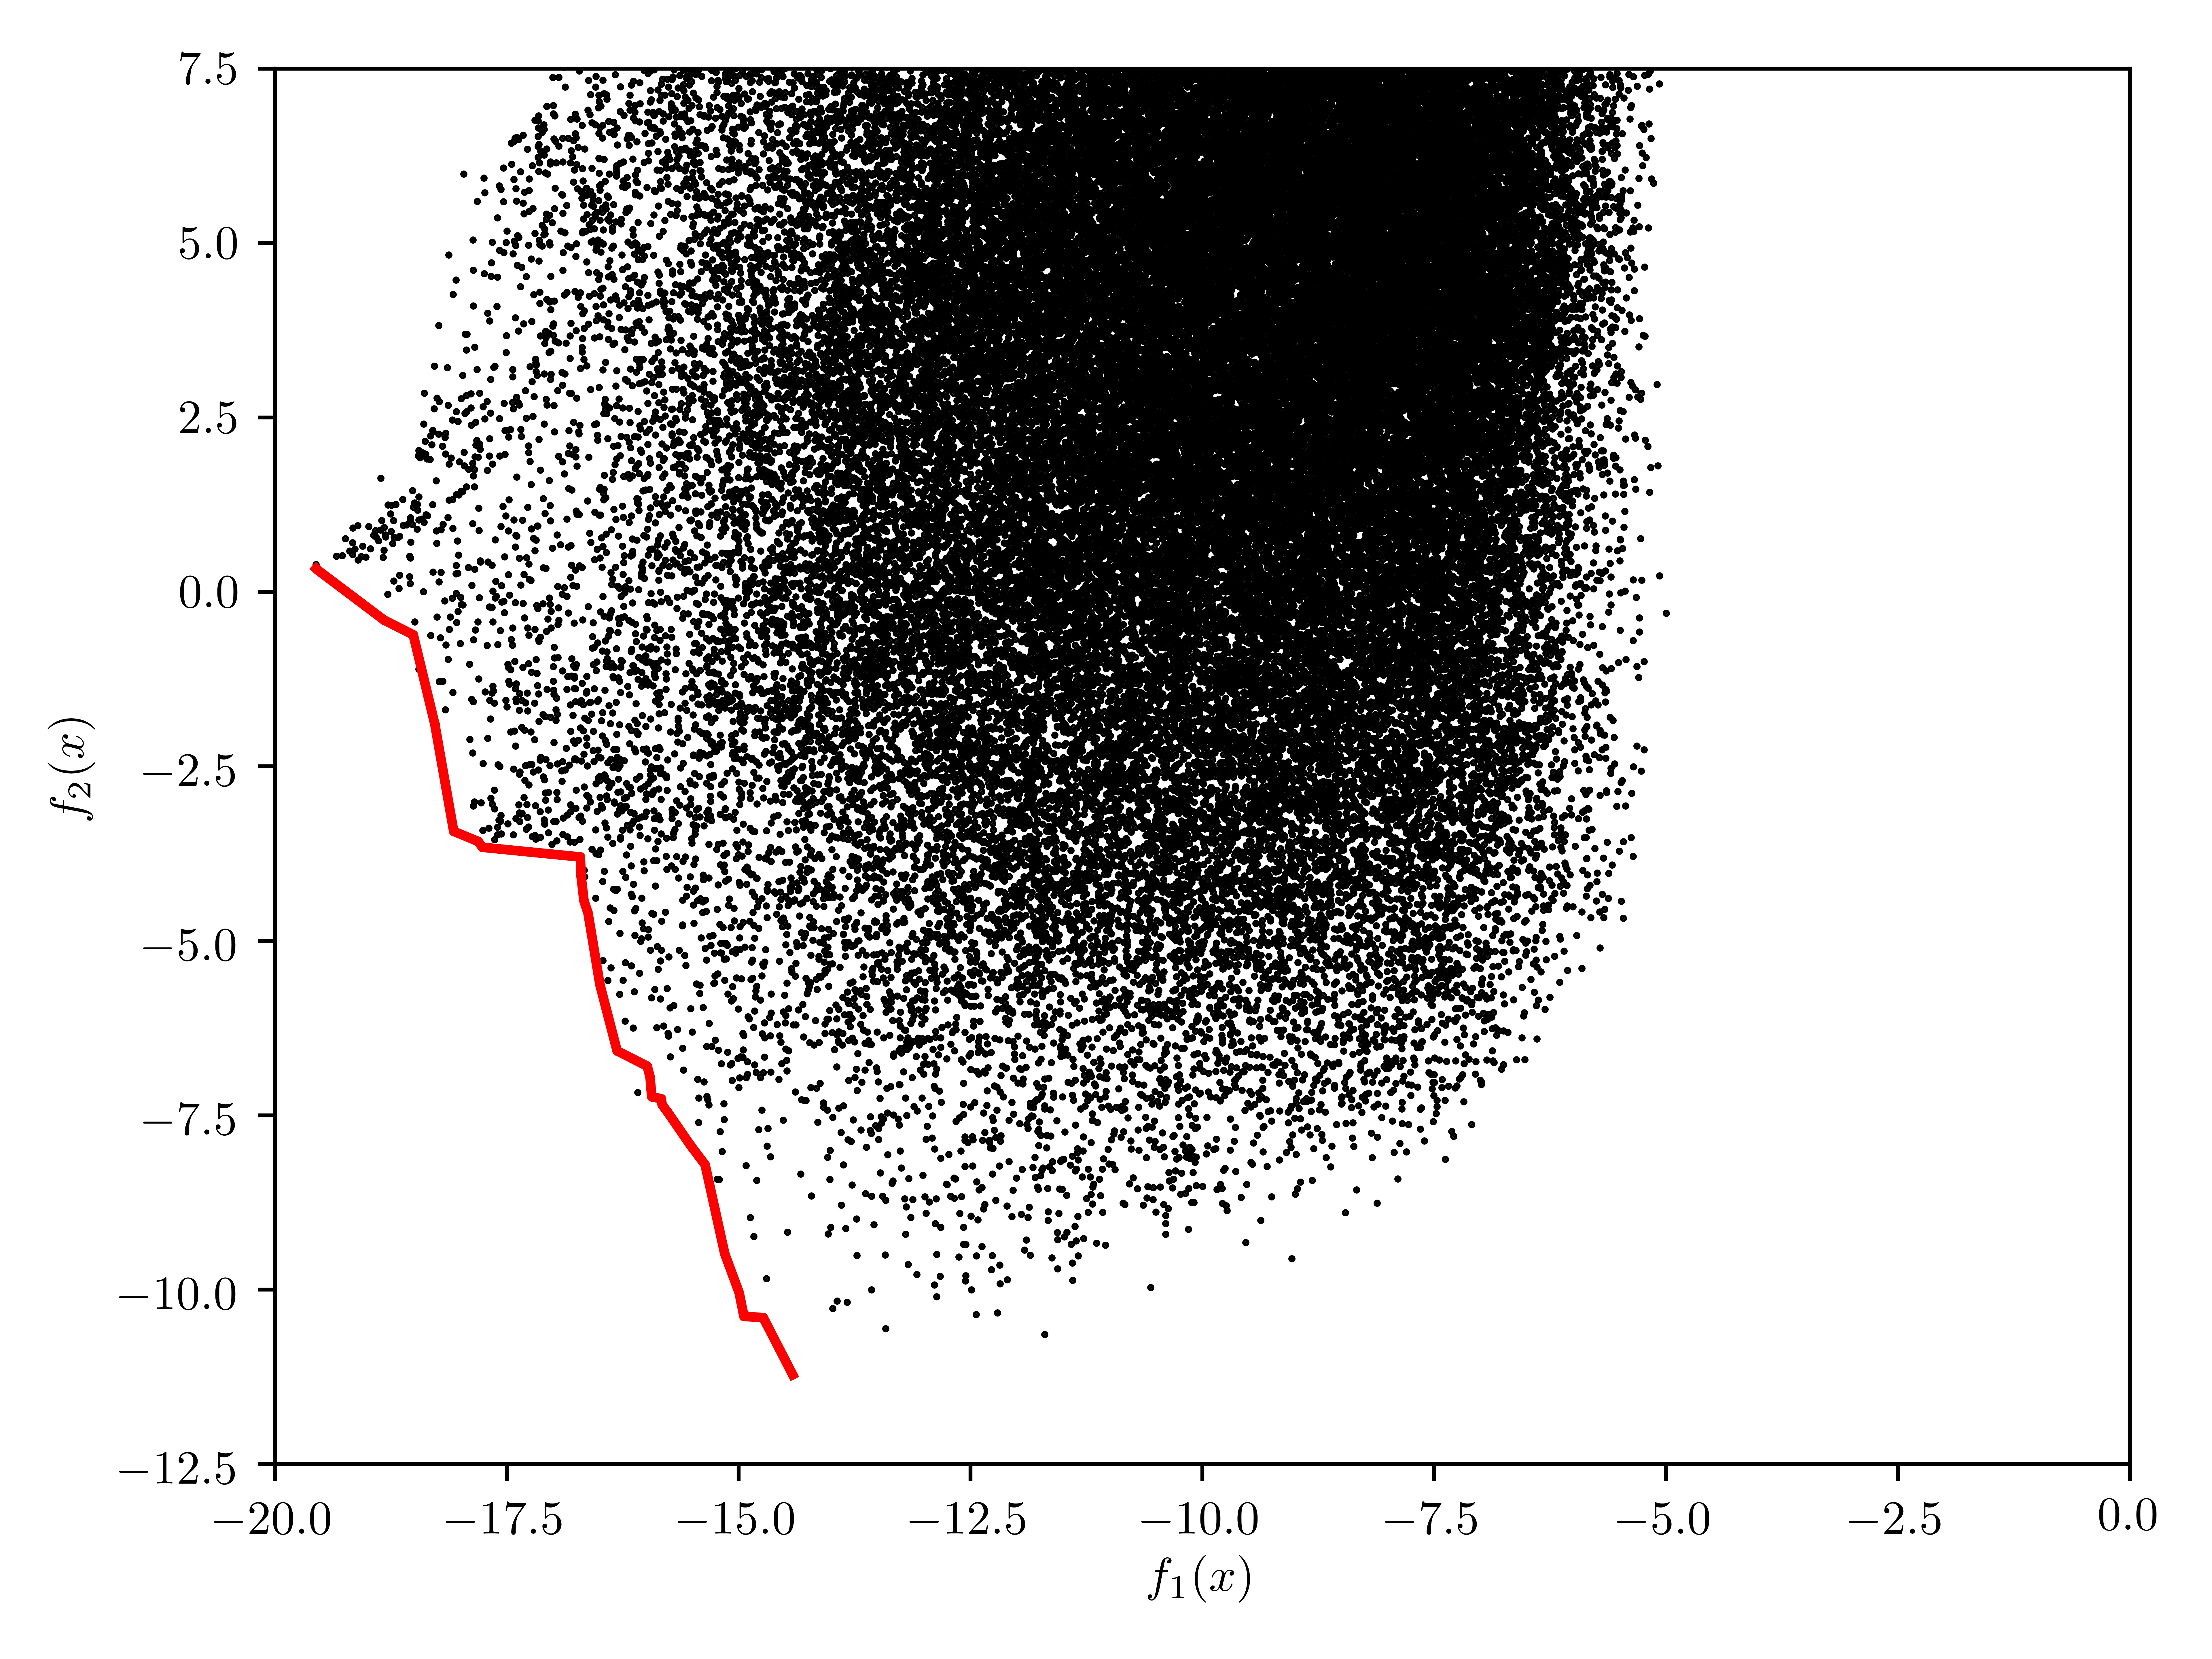
\includegraphics{chapter3/kurasawe_mc}
  \caption{Results of the MC strategy to estimate the Pareto surface.  Black point are the results of the dominated function evaluation of $x$, while the Pareto optimal function evaluation are denoted in red.}
  \label{fig:kurasawe_mc}
\end{figure}

Figure \ref{fig:kurasawe_mc} provides the simulation results of the MC strategy.   As expected with a non-informative distribution, the majority of function evaluations of $x$ results in results far away from the Pareto optimal surface denoted red.  Unlike the CG strategy, this strategy is able to estimate convex regions of the Pareto curve.

\begin{figure}[htbp]
	\centering
  \includegraphics{chapter3/kurasawe_kde}
  \caption{Results of the last iteration of the KDE strategy to estimate the Pareto surface.  Black point are the results of the dominated function evaluation of $x$, while the Pareto optimal function evaluation are denoted in red.}
  \label{fig:kurawawe_kde}
\end{figure}

Figure \ref{fig:kurawawe_kde} provides the simulation results of the KDE strategy.  Here, only the results of the final iteration are displayed.  In the last iteration, the evolved probability distribution function samples point close to Pareto curve.  While the number of Pareto points wich the MC strategy (N=311) and the KDE strategy (N=508) are of the same order of magnitude, the resolution quality of the Pareto surface for the KDE strategy is clearly superior.

\begin{figure}[htbp]
	\centering
  \includegraphics{chapter3/kurasawe_comparison}
  \caption{Comparative comparison of the Pareto surface for the CG, MC, and KDE strategies.}
  \label{fig:kurasawe_comparison}
\end{figure}

Figure \ref{fig:kurasawe_comparison} overlays the Pareto surfaces and points for each strategy into the same chart for qualitative comparison.  When the CG strategy is compared to the Monte Carlo sampling strateges (MC and KDE), the deficiencies of the local optimization strategies becomes apparent.  The cost function is unable to resolve regions of the Pareto surface which are occluded in a convex region.  The CG method is only able to identify two regions of relative spare density in the lower right quadrant, where there is clear concave regions to converge to.

In some cases, the CG method identifies potential parameterization which dominate solutions identified by the MC and KDE schemes.  With an appropriate choice of initial conditions and weights, the gradient based optimization scheme CG can converge solutions to the Pareto surface with abitrary solutions.  This suggests that Monte Carlo strategies are complementary to conventional potential optimization approaches.

The MC and KDE strategies have qualitatively similar results.  Since these optimization algorithms are not burdened with a cost function, they are able to identify convex regions of the Pareto surface.  The KDE has superior resolution quality in determining the Pareto curve, due to update of the probability density function.

The results of this demonstration have clear implications on the choice of optimization algorithms for potential development.  The typical appproach to potential development are likely inadequate.  The high sensitivity of QOI predictions with respect to small changes in weights is indicative that there are regions of compromise solutions which are Pareto optimal, but not identifiable by with current results.

Moreover, the CG strategy automates an \emph{ad hoc} variation of initial conditions and weighting schemes consistent with current approaches.  Concerns about the convergence of Monte Carlo style sampling schemes should be reconsidered in light  of the fact that the presence of convexity and local minima imposes a high computational cost measured in total function evaluations.

%The strength of the KDE strategy shows initial promise as an optimization technique, and should not be compared to scalar global optimizers.  Scalar global optimizers are cardinal optimization methods, while our strategy is an ordinal optimization method.  The sampling region of cardinal optimization methods only improves when a new optima is achieved.  In ordinal optimization methods, the sampling efficiency improves whenever a new Pareto point is identified.
